\documentclass{ctexart}
\usepackage{geometry}
\usepackage{fancyhdr}
\usepackage{graphicx}
\usepackage{booktabs}
\usepackage{amsmath}
\usepackage{caption}
\usepackage{multirow}
\usepackage{tikz}
\usepackage{array}
\xeCJKsetup{CJKmath=true} 
\usepackage{zhnumber} % change section number to chinese
\renewcommand\thesection{\zhnum{section}}
\renewcommand \thesubsection {\arabic{subsection}}
\CTEXsetup[format={\Large\bfseries}]{section}

\geometry{
    a4paper,
    left=3.18cm,
    right=3.18cm,
    top=3.04cm,
    bottom=3.04cm
}

\pagestyle{fancy}
\fancyhf{}
\renewcommand{\headrulewidth}{0.7pt} % 设置页眉横线粗细
\fancyhead[L]{\kaishu\large 大学物理实验报告} % 在左侧设置页眉文字
\fancyhead[R]{\kaishu\large 哈尔滨工业大学(深圳) } % 在右侧设置页眉文字
\fancyfoot[R]{\thepage} % 将页数放在右下角


\setlength\headwidth{\textwidth}

\begin{document}

\noindent
\textbf{
    \begin{tabular}{p{2.4cm}p{2.4cm}p{4cm}p{3.8cm}}
        班级 \hrulefill & 学号 \hrulefill & 姓名 \hrulefill & 教师签字 \hrulefill \\
    \end{tabular}\\
    \begin{tabular}{p{6cm}p{3.6cm}p{3.55cm}}
        \ 实验日期 \hrulefill & 预习成绩 \hrulefill & 总成绩 \hrulefill
    \end{tabular}\\
}
\rule[-10pt]{\textwidth}{0.7pt}

\begin{center}
    \Large \textbf{实验内容 \underline{自组光栅光谱仪实验}}
\end{center}

\section{预习内容}

\subsection{请绘制Czerny-Turner(C-T)光谱仪的主要光路图。}

\vspace{10\baselineskip}

\subsection{请简述光栅分光原理。}

\vspace{10\baselineskip}

\subsection{光谱仪中的重要参数—分辨率和色散率如何定义?}

\newpage
\section{实验现象及原始数据记录}

\subsection{自组光栅光谱仪的搭建(附搭建完成后的照片)}

\begin{figure}[!h]
    \centering
    \caption{自组光栅光谱仪搭建照片}
    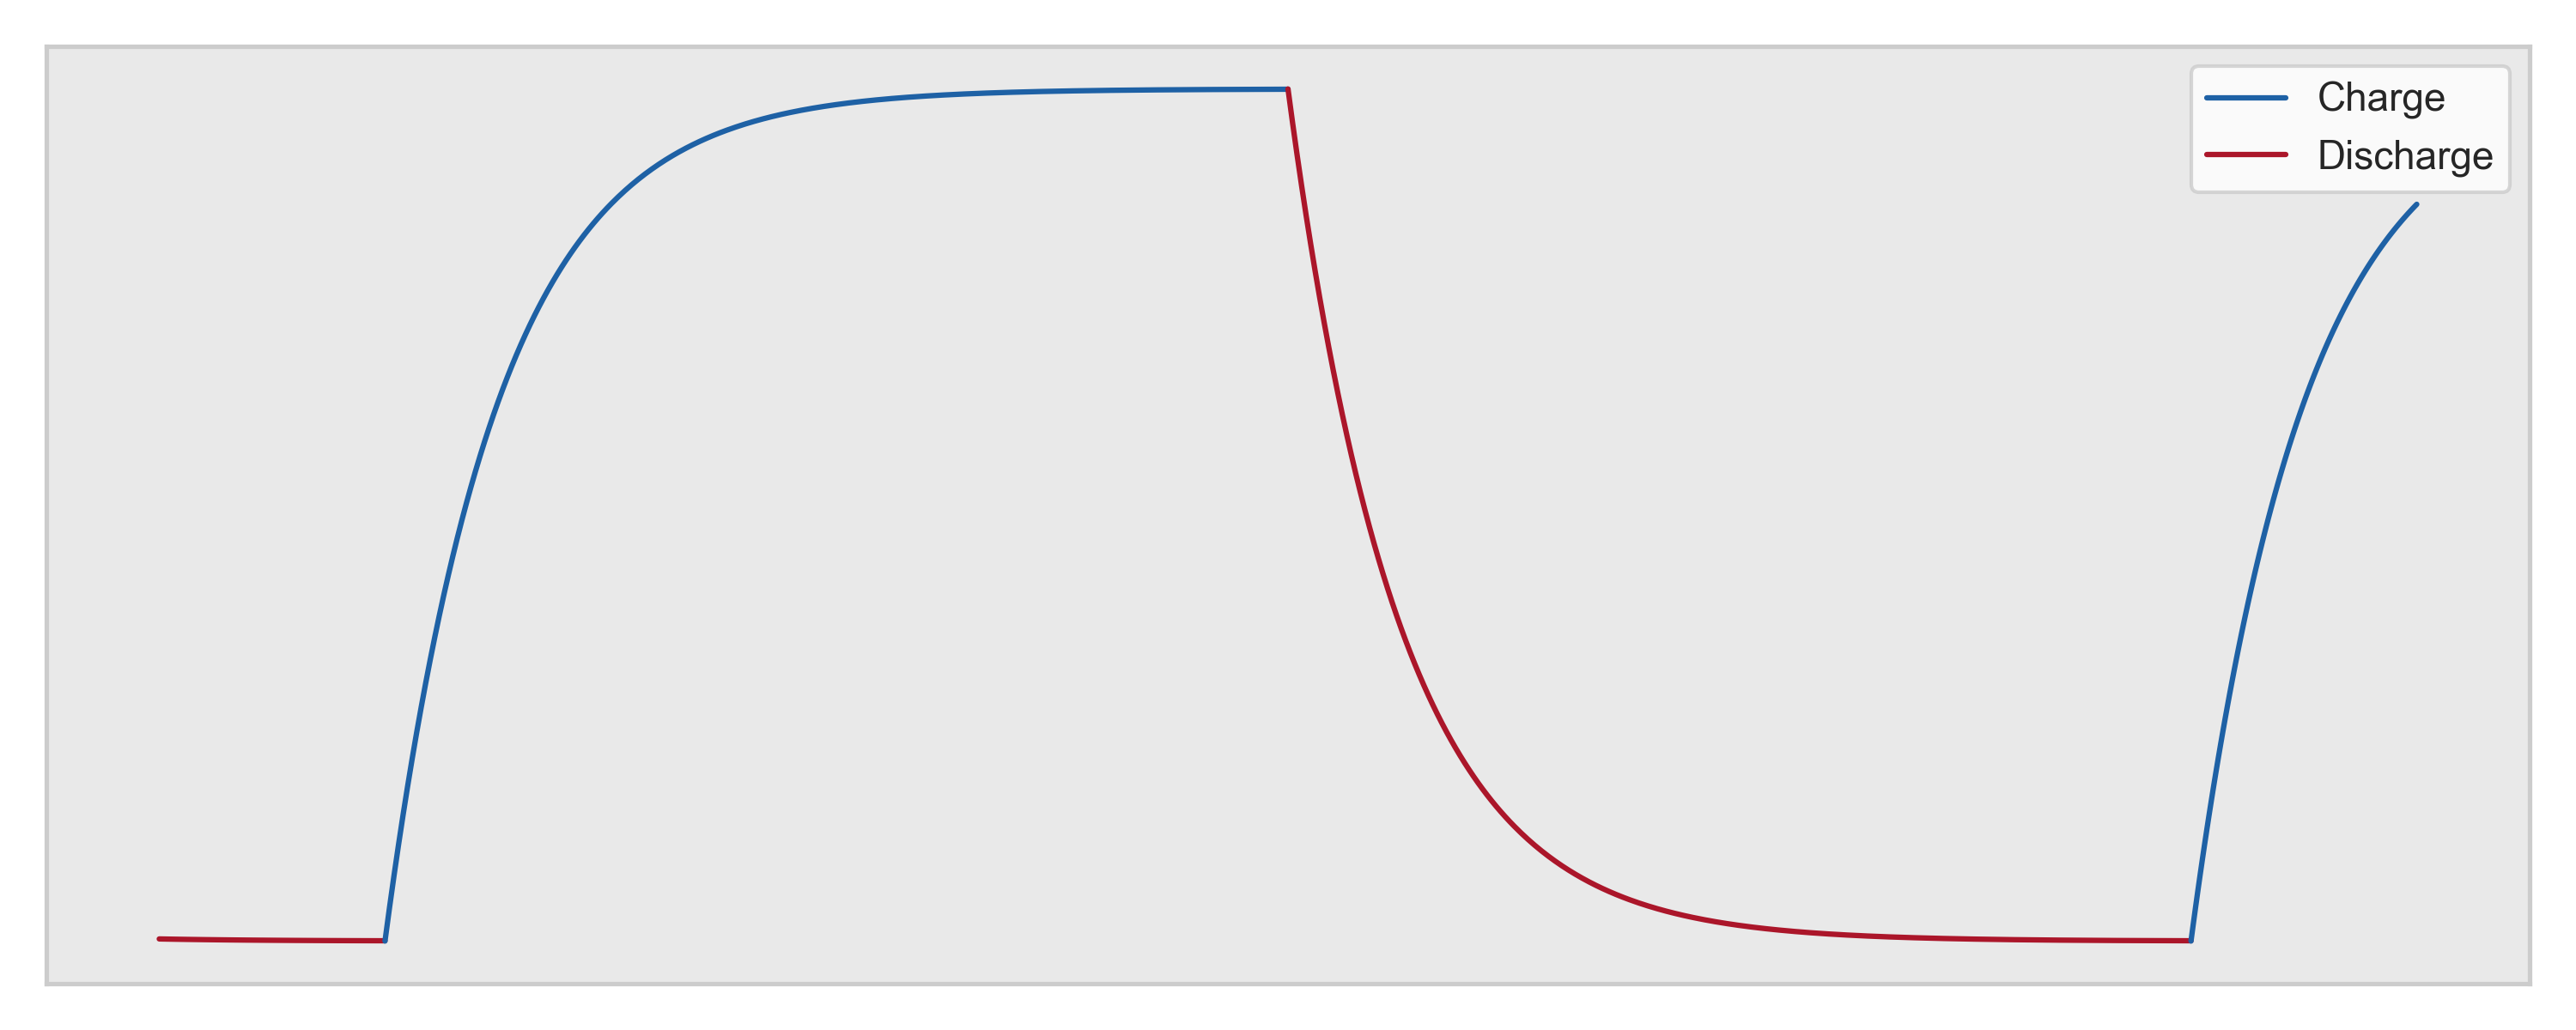
\includegraphics[width=0.8\textwidth]{pic.png}
\end{figure}

\subsection{Hg灯光谱和光栅光谱仪的标定}

记录汞灯光谱,并将主要数据记录在表格 1中,并由此进行标定,得到光谱仪的标定方程,最后通过测试软件将像素坐标转化为波长坐标。

\begin{figure}[!htbp]
    \centering
    \caption{Hg灯光谱原始图像(未标定)}
    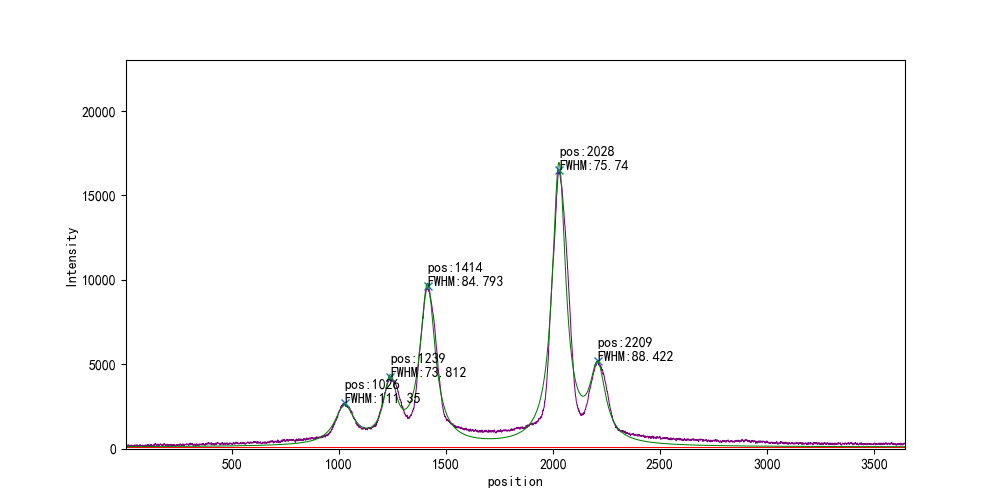
\includegraphics[width=\textwidth]{raw.png}
\end{figure}

\newpage

\begin{table}
    \renewcommand{\arraystretch}{1.3}
    \centering
    \caption{汞灯光谱数据记录表}
    \begin{tabular}{|m{2.3cm}<{\centering}|m{2.5cm}<{\centering}|m{2.3cm}<{\centering}|m{2.3cm}<{\centering}|}
        \hline
        汞灯谱线波长$\lambda(nm)$ & CCD像素位置 (pixels) & FWHM (pixels) & FWHM \ \ \ (nm) \\
        \hline
        365.48 &  &  & \\
        \hline
        404.66 &  &  & \\
        \hline
        435.84 &  &  & \\
        \hline
        546.07 &  &  & \\
        \hline
        576.96 & \multirow{2}*{} & \multirow{2}*{} & \multirow{2}*{} \\
        \cline{1-1}
        579.07 &  &  & \\
        \hline
    \end{tabular}
\end{table}


\begin{tikzpicture}[remember picture,overlay]
    \node[anchor=south east,inner sep=100pt] at (current page.south east) {
        \renewcommand{\arraystretch}{1.5} % 表格行高倍数
        \setlength{\tabcolsep}{18pt}    
    \begin{tabular}{|c|c|}
        \hline
        \LARGE  教师 & \LARGE  姓名 \\
        \hline
        \LARGE \kaishu 签字 &  \\
        \hline
        \end{tabular}
    };
\end{tikzpicture}

\newpage

\section{实验数据处理}

\subsection{标定后的Hg的光谱图}

\begin{figure}[!htbp]
    \centering
    \caption{标定Hg灯光谱}
    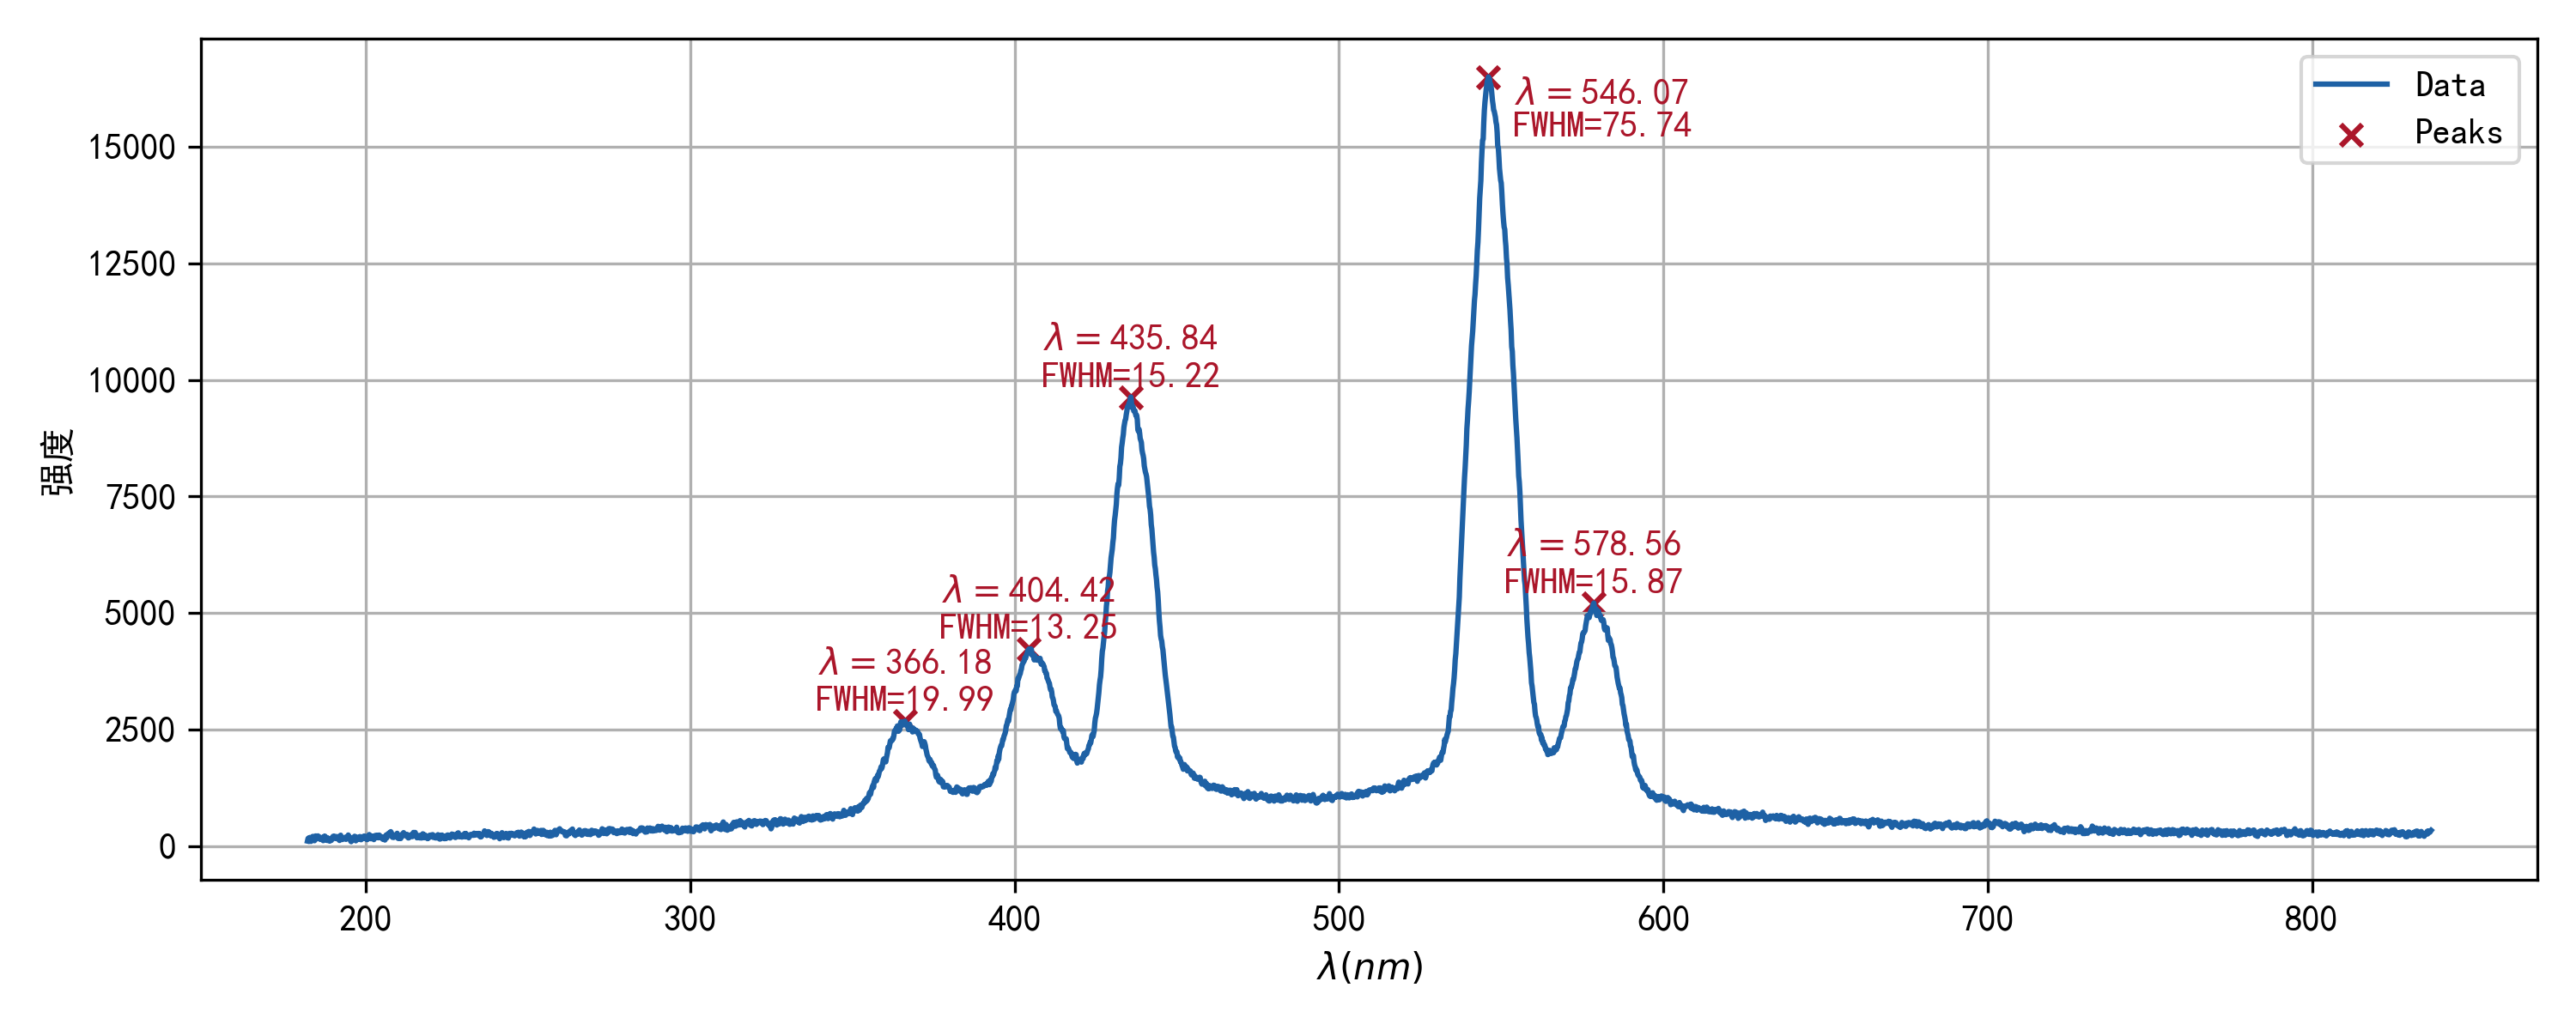
\includegraphics[width=\textwidth]{result.png}
\end{figure}

\section{讨论题}

\subsection{如何提高光栅光谱仪的分辨率?}

首先,增大光栅的刻线密度能增强对不同波长的分离效果,使相邻波长更易区分。但是这是不现实的,因为光栅的刻线密度是固定的。

除此之外,通过狭缝调节器或聚光镜缩窄入射光束宽度,可以减少重叠干扰,提升分辨能力。同时,增加光程长度,即扩大光栅与探测器间的距离,可使不同波长的光在探测器上更加清晰地分开。此外,精确调整光栅的倾角,使其更符合布拉格条件,能够使光谱分离更加明显。若使用更大的光栅面积,也能增大有效区域,提升光谱清晰度。最后,采用高分辨率探测器能精确捕捉光谱分布,尤其是小像素探测器,可以更清晰地分辨相邻波长。通过以上改进,光栅光谱仪的分辨率将显著提升,使其能够更精确地检测到波长间的微小差异。

\subsection{光栅光谱仪的应用有哪些?}

光栅光谱仪在许多科学研究和工业应用中扮演着关键角色。首先,在物理和化学分析中,它被广泛用于分子和原子的光谱分析,通过解析样品的吸收或发射光谱,确定物质成分及其浓度。其次,光栅光谱仪在环境监测中发挥重要作用,用于检测空气、水和土壤中的污染物,尤其是痕量的气体和金属成分。此外,在天文学中,光栅光谱仪被用来研究星体的光谱,分析恒星和星系的化学组成、温度、速度等信息,为探索宇宙提供了重要数据支持。该设备还在生命科学领域应用广泛,如医学诊断中的血液分析、食品和药物的质量检测等。最后,光栅光谱仪在工业质量控制中也很重要,可用于检测材料的光学特性、表面瑕疵以及薄膜的厚度,从而确保产品的质量与一致性。

\end{document}